% Created 2022-07-08 Fri 11:51
% Intended LaTeX compiler: pdflatex
\documentclass[presentation,aspectratio=1610]{beamer}
\usepackage[utf8]{inputenc}
\usepackage[T1]{fontenc}
\usepackage{graphicx}
\usepackage{grffile}
\usepackage{longtable}
\usepackage{wrapfig}
\usepackage{rotating}
\usepackage[normalem]{ulem}
\usepackage{amsmath}
\usepackage{textcomp}
\usepackage{amssymb}
\usepackage{capt-of}
\usepackage{hyperref}
\usepackage{khpreamble}
\usepackage{amssymb}
\DeclareMathOperator{\shift}{q}
\DeclareMathOperator{\diff}{p}
\usetheme{default}
\author{Kjartan Halvorsen}
\date{2022-07-08}
\title{Discretizing continuous-time controllers}
\hypersetup{
 pdfauthor={Kjartan Halvorsen},
 pdftitle={Discretizing continuous-time controllers},
 pdfkeywords={},
 pdfsubject={},
 pdfcreator={Emacs 26.3 (Org mode 9.4.6)}, 
 pdflang={English}}
\begin{document}

\maketitle


\section{Intro}
\label{sec:org3cfdf55}

\section{Discretization}
\label{sec:org4173e32}
\begin{frame}[label={sec:orge7a4022}]{Context}
\begin{itemize}
\item Controller \(F(s)\) obtained from a design in continuous time.
\item Need discrete approxmation in order to implement on a computer
\end{itemize}

\begin{center}
 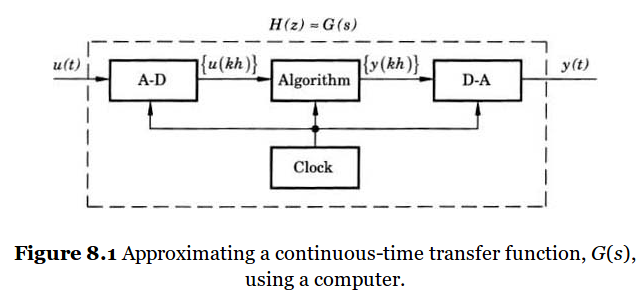
\includegraphics[width=0.7\linewidth]{../../figures/fig8-1.png}\\
 \footnotesize Source: Åström \& Wittenmark 
\end{center}
\end{frame}

\section{Warm-up: Differentiation}
\label{sec:org78c256d}

\begin{frame}[label={sec:org31a75f1}]{Warm-up exercise}
\begin{columns}
\begin{column}{0.4\columnwidth}
\begin{center}
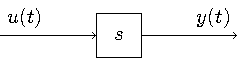
\includegraphics[width=\linewidth]{../../figures/block-simple-derivative}
\end{center}

\alert{Draw the Bode diagram for the transfer function}
\end{column}
\begin{column}{0.6\columnwidth}
\begin{center}
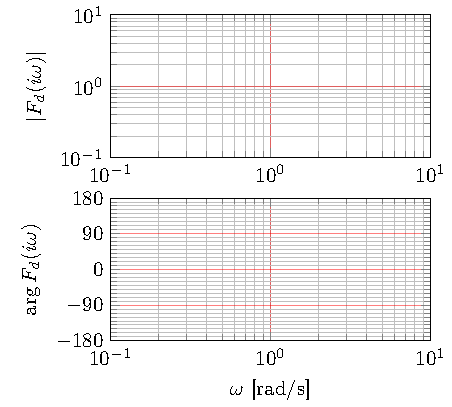
\includegraphics[width=\linewidth]{../../figures/bode-derivative-empty}
\end{center}
\end{column}
\end{columns}
\end{frame}

\begin{frame}[label={sec:orge36f0a5}]{Discrete-time differentiation}
\begin{center}
\begin{tabular}{lll}
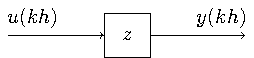
\includegraphics[width=0.3\linewidth]{../../figures/block-simple-shift-z} & \(\Leftrightarrow\) & 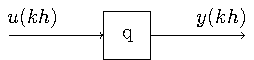
\includegraphics[width=0.3\linewidth]{../../figures/block-simple-shift}\\
\end{tabular}
\end{center}



\begin{columns}
\begin{column}{0.4\columnwidth}
\vspace*{5mm}

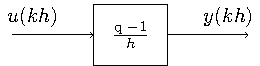
\includegraphics[width=\linewidth]{../../figures/block-simple-discrete-derivative-fwd}

\textcolor{white}{Space}

\begin{center}
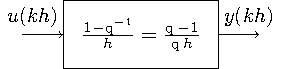
\includegraphics[width=\linewidth]{../../figures/block-simple-discrete-derivative}
\end{center}
\end{column}

\begin{column}{0.6\columnwidth}
\begin{align*}
y(kh) &= \frac{\shift-1}{h} u(kh) = \frac{\shift u(kh) - u(kh)}{h}\\ &= \frac{u(kh + h) - u(kh)}{h}\\\\
&\textcolor{white}{hej}
\end{align*}
\end{column}
\end{columns}
\end{frame}

\begin{frame}[label={sec:org1066e7b}]{Discretization methods}
\begin{enumerate}
\item Forward difference. Substitute 
\[ s = \frac{z-1}{h} \] in \(F(s)\) to get
\[ F_d(z) = F(s')|_{s'=\frac{z-1}{h}}. \]
\item Backward difference. Substitute 
\[ s = \frac{z-1}{zh} \] in \(F(s)\) to get
\[ F_d(z) = F(s')|_{s'=\frac{z-1}{zh}}. \]
\end{enumerate}
\end{frame}
\begin{frame}[label={sec:org35f1812}]{Discretization methods, contd.}
\begin{enumerate}
\setcounter{enumi}{2}
\item Tustin's method (also known as the bilinear transform). Substitute
\[ s = \frac{2}{h}\frac{z-1}{z+1} \] in \(F(s)\) to get
\[ F_d(z) = F(s')|_{s'=\frac{2}{h}\cdot \frac{z-1}{z+1}}. \]
\item Ramp invariance. This is similar to ZoH, which is step-invariant approximation. 
Since a unit ramp has z-transform \(\frac{zh}{(z-1)^2}\) and Laplace-transform \(1/s^2\),  the discretization becomes
\[ F_d(z) = \frac{(z-1)^2}{zh} \ztrf{\laplaceinv{\frac{F(s)}{s^2}}}. \]
\end{enumerate}
\end{frame}

\begin{frame}[label={sec:org09330e0}]{Frequency warping using Tustin's}
\begin{center}
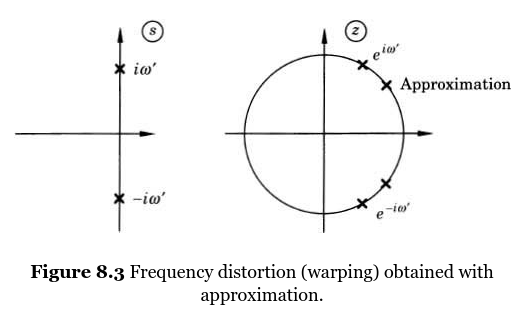
\includegraphics[width=0.6\linewidth]{../../figures/fig8_3.png}
\end{center}
The infinite positive imaginary axis in the s-plane is mapped to the finite-length upper half of the unit circle in the z-plane.
\end{frame}
\begin{frame}[label={sec:org77f91c0}]{Forward difference exercise}
\begin{center}
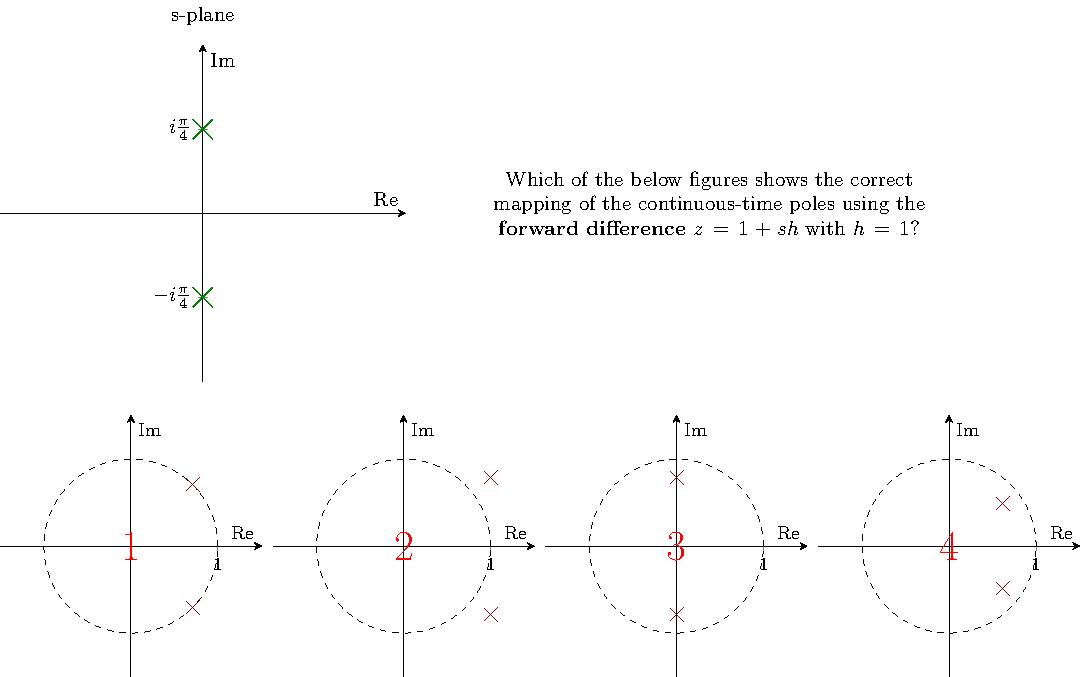
\includegraphics[width=\linewidth]{../../figures/forward-diff-exercise}
\end{center}
\end{frame}

\begin{frame}[label={sec:org1437175}]{Backward difference exercise}
\begin{center}
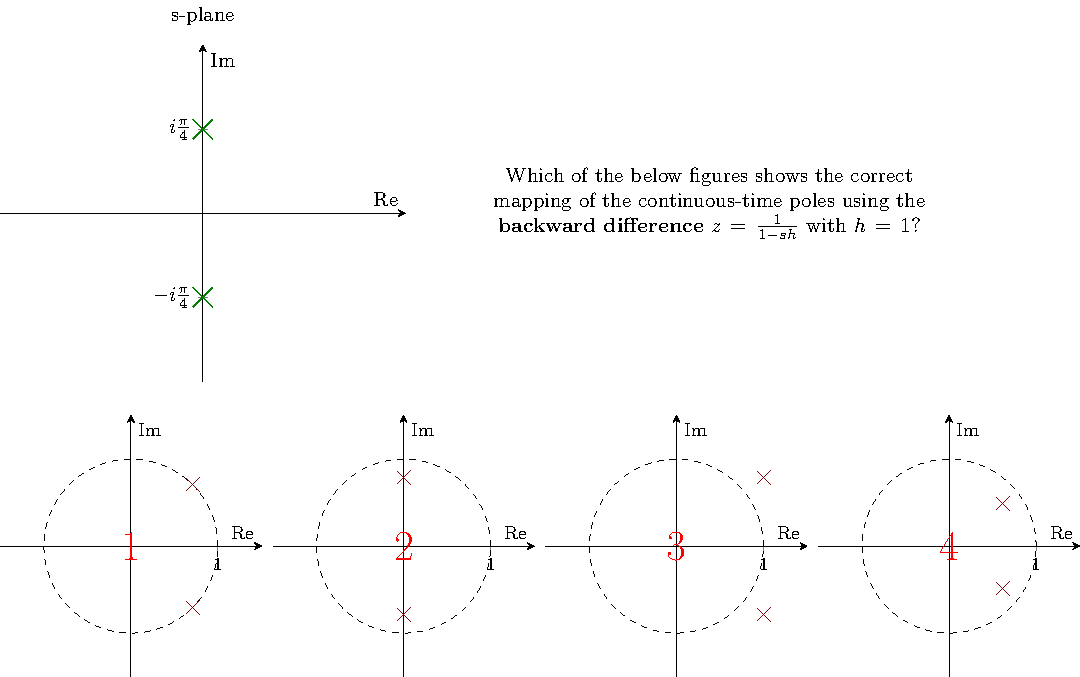
\includegraphics[width=\linewidth]{../../figures/backward-diff-exercise}
\end{center}
\end{frame}


\begin{frame}[label={sec:org47c0825}]{Bilinear transformation exercise}
\begin{center}
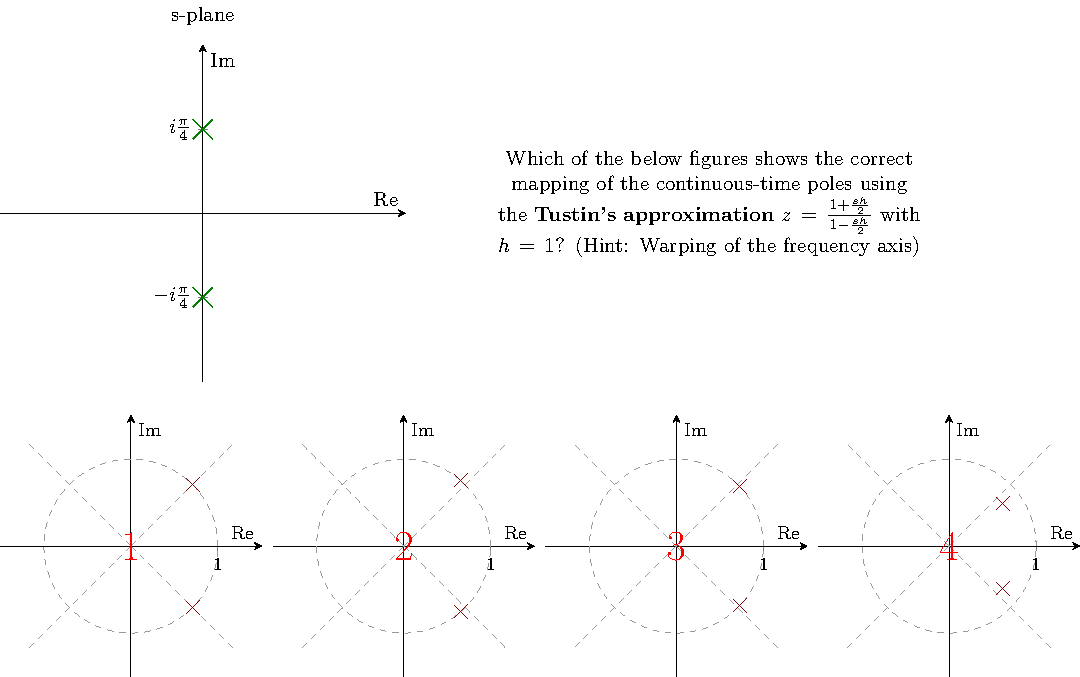
\includegraphics[width=\linewidth]{../../figures/tustin-diff-exercise}
\end{center}
\end{frame}
\end{document}